\scanpage{39}
Maintenant on déduit donc des isom
\[
(46)\qquad\left\{\begin{aligned}
\pi_\infty&\simeq\widehat{\mathbb Z}^{\,3}/\widehat{\mathbb Z}\\
\deleted{\unsure{\mathcal E\simeq(\mathfrak S_3\times\widehat{\mathbb Z}^{*})/\widehat{\mathbb Z}}}&\\
\mathcal E&\simeq
\underbrace{(\unsure{\mathfrak S_3|\mathbb G_3}\times\Gamma)}_{
\substack{\text{opérant via}\\\text{permutation des}\\\text{facteurs et}\\
\text{via homothéties}\\\text{par }\chi:\Gamma\longrightarrow\widehat{\mathbb Z}^{*}}}
\mathbin{\underset{\scriptscriptstyle1/2}{.}}
(\widehat{\mathbb Z}^{\,3}/\widehat{\mathbb Z})
\end{aligned}\right.
\]
\inserted{\figure{\begin{tikzpicture}
\node at (0,0) {$\pi_n\simeq(\mathbb Z/n)^3/\mathbb Z_n$};
\draw (0,0) ellipse (2.5cm and .65cm);
\draw[->] (2.5,0).. controls (4,.1) and (4,1.5)..(3.7,3.2);
\end{tikzpicture}}}
\[
(47)\qquad\alpha_\infty\simeq(-1,+1,0)\bmod\widehat{\mathbb Z}
\qquad\text{d'où}
\]
\[
(47')\qquad\alpha'_\infty=\overline\alpha_\infty
=(1,-1,0)\bmod\widehat{\mathbb Z}
\]
Considérons les éléments
\[
(48)\qquad\left\{\begin{aligned}
&\rho_0,\rho_1,\rho_\infty\in\pi_\infty\\
&\rho_0=(1,0,0)\bmod\widehat{\mathbb Z}\\
&\rho_1=(0,1,0)\quad\text{---}\\
&\rho_\infty=(0,0,1)\quad\text{---}
\end{aligned}\right.
\]
de sorte que
\[
(49)\qquad\rho_0\rho_1\rho_\infty=1
\]
\margin{\figure{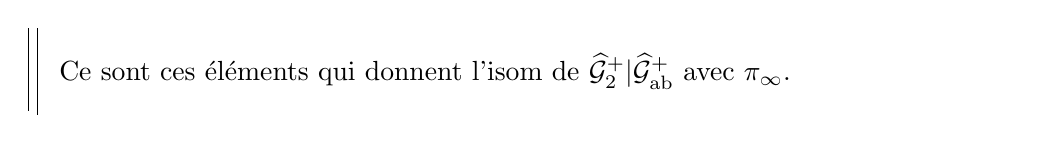
\begin{tikzpicture}
\node[anchor=west,text width=12cm] at (0,0) {Ce sont ces éléments qui donnent l'isom de
$\unsure{\widehat{\mathcal G}_2^+|\widehat{\mathcal G}_{\mathrm{ab}}^+}$
avec $\pi_\infty$.};
\draw (-.15,-.55)--(-.15,.55);
\draw (-.27,-.5)--(-.27,.55);
\end{tikzpicture}}}
% archive foliation: 38
